\section{Motivation}
\begin{frame}[plain, c]
    \begin{center}
        \Huge \textcolor{NavyBlue}{\textbf{Motivation}}
    \end{center}
\end{frame}

\begin{frame}
    \frametitle{Theoretical Motivation}
    \begin{itemize}
        \item Black-box objective functions are functions that we can only
                interact with via its inputs and outputs meaning typical
                methods don't work.
        \item Expensive-to-evaluate objective functions are functions that
                require significant effort to obtain outputs but can be
                approximated and modeled using the Bayesian approach.
        \item Useful when objectives lack analytical evaluation.
        \item Useful when objectives have no efficient (if it exists) gradient.
    \end{itemize}
\end{frame}

\begin{frame}
    \frametitle{Applications}
    The application potential of Bayesian optimization can be seen across
    several critical domains, especially those attempting to accelerate finding
    solutions to real-world scientific and engineering problems.

    \vspace*{6pt}
    \begin{itemize}
        \item Drug Discovery
        \item Molecule/Protein Discovery
        \item Materials Design
        \item AutoML (hyperparameter tuning)
        \item Engineering Decisions
        \item Many more...
    \end{itemize}
\end{frame}

\begin{frame}
    \frametitle{Application: Drug Discovery}
    \begin{figure}
        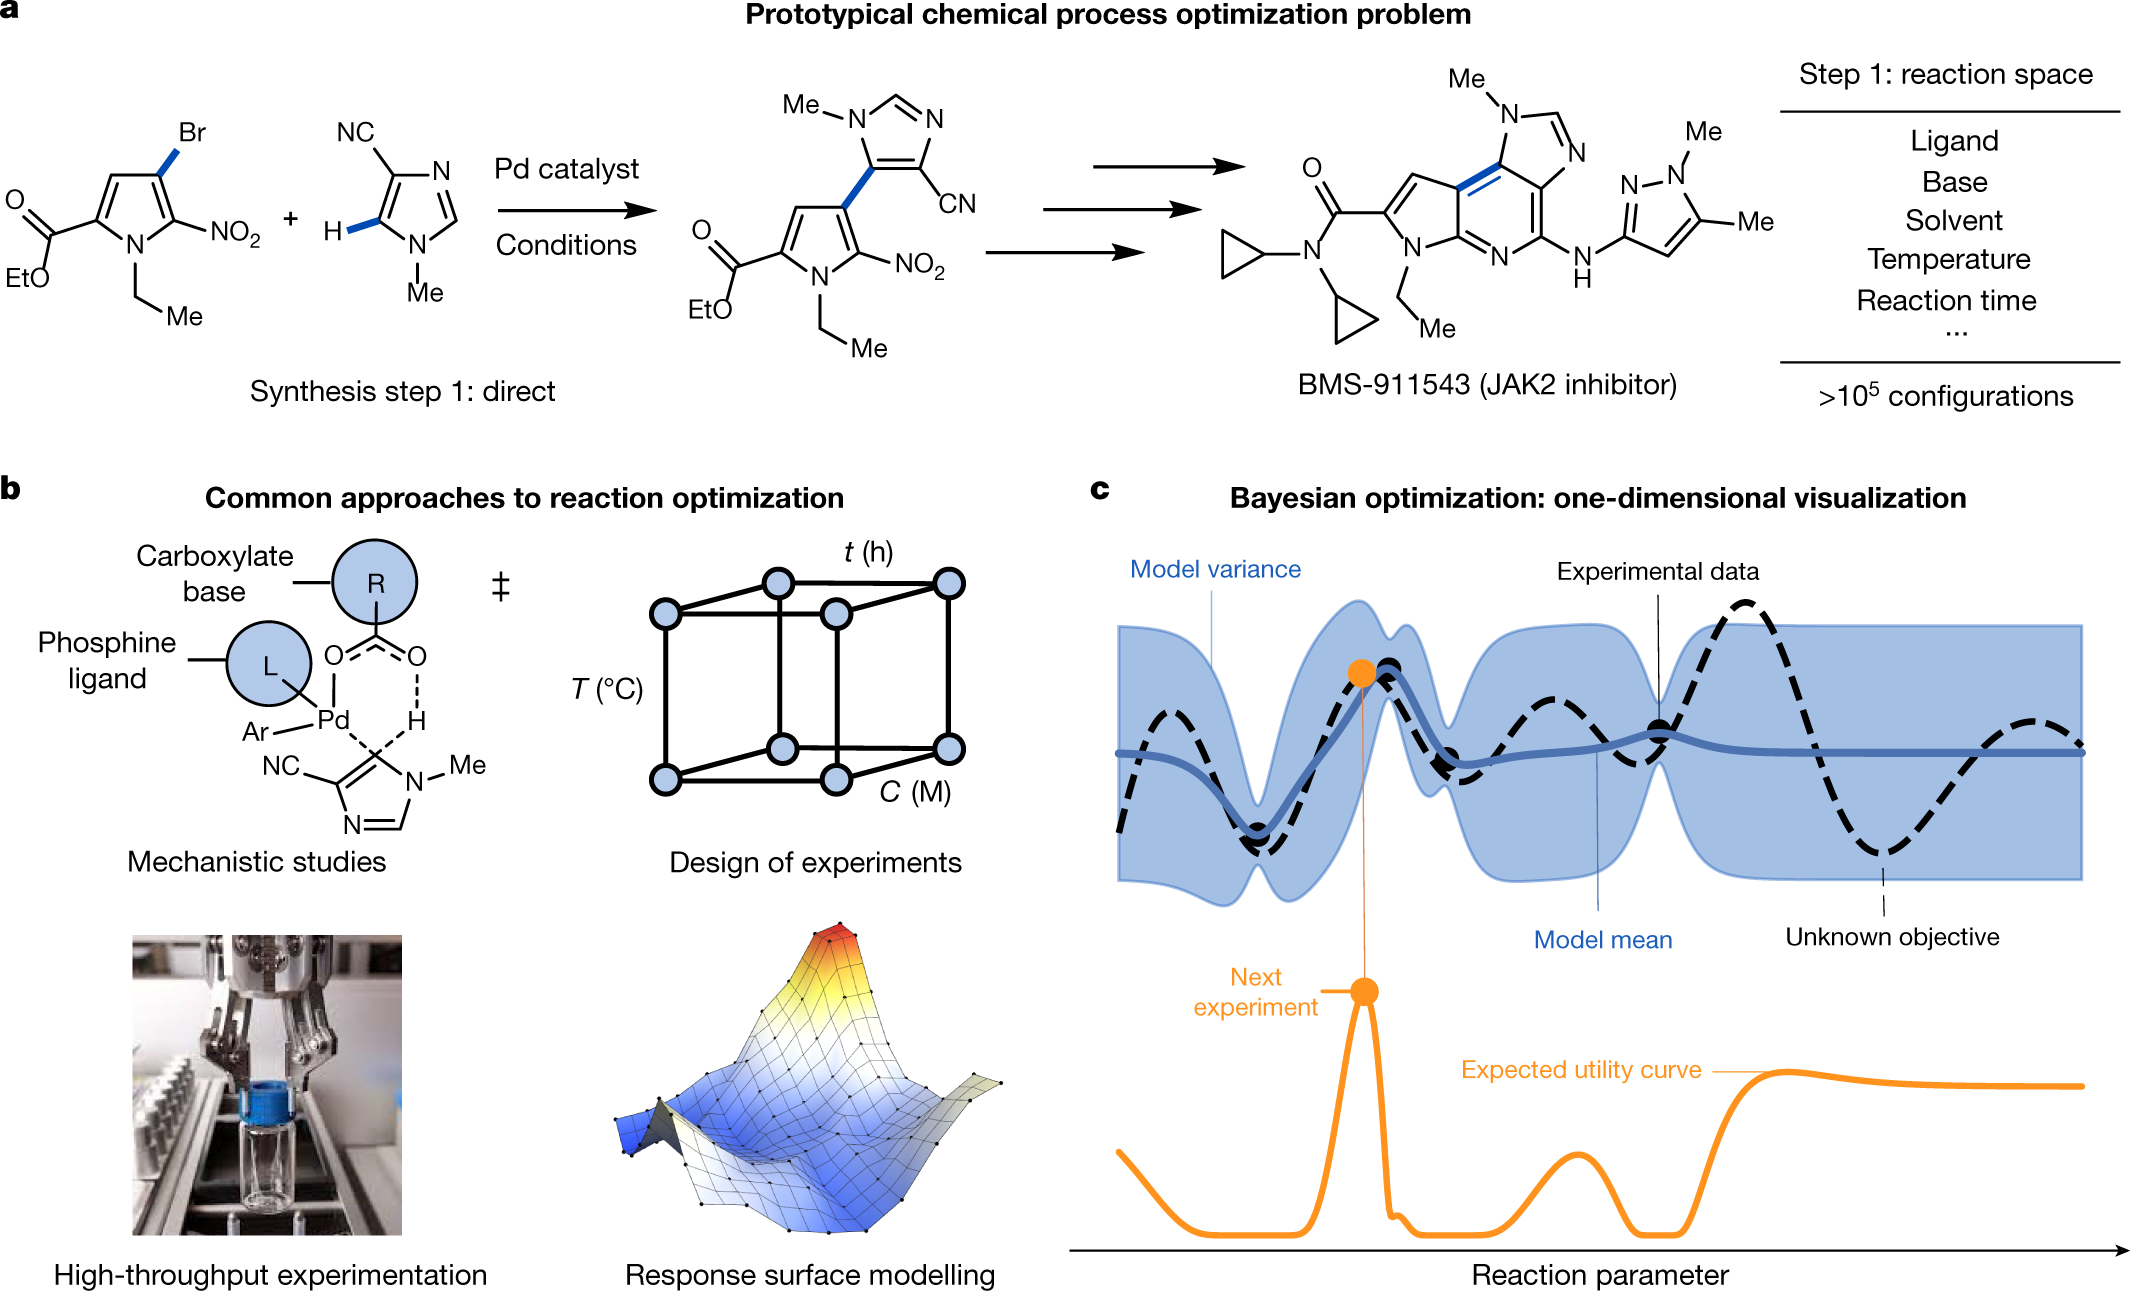
\includegraphics[width=0.75\textwidth]
            {content/graphics/applications/drug-discovery.png}
        \caption{Overview of Drug Synthesis from \emph{Bayesian optimization as
            a tool for chemical synthesis} by Shields et al. (2021)}
    \end{figure}
\end{frame}

\begin{frame}
    \frametitle{Application: Molecule/Protein Discovery}
    \begin{figure}
        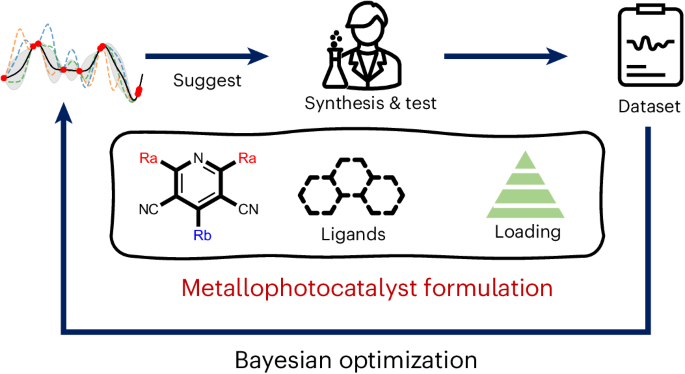
\includegraphics[width=0.75\textwidth]
            {content/graphics/applications/molecule-protein-discovery.png}
        \caption{Closed Loop for Molecular Discovery from \emph{Sequential
            closed-loop Bayesian optimization as a guide for organic molecular
            metallophotocatalyst formulation discovery} by Li et al. (2024)}
    \end{figure}
\end{frame}

\begin{frame}
    \frametitle{Application: Materials Discovery}
    \begin{figure}
        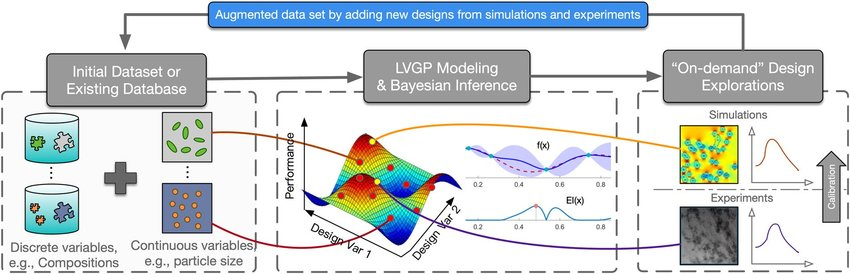
\includegraphics[width=\textwidth]
            {content/graphics/applications/materials-design.jpg}
        \caption{Material Design Framework from \emph{Bayesian Optimization for
            Materials Design with Mixed Quantitative and Qualitative Variables}
            by Zhang et al. (2020)}
    \end{figure}
\end{frame}

\begin{frame}
    \frametitle{Application: AutoML}
    \begin{figure}
        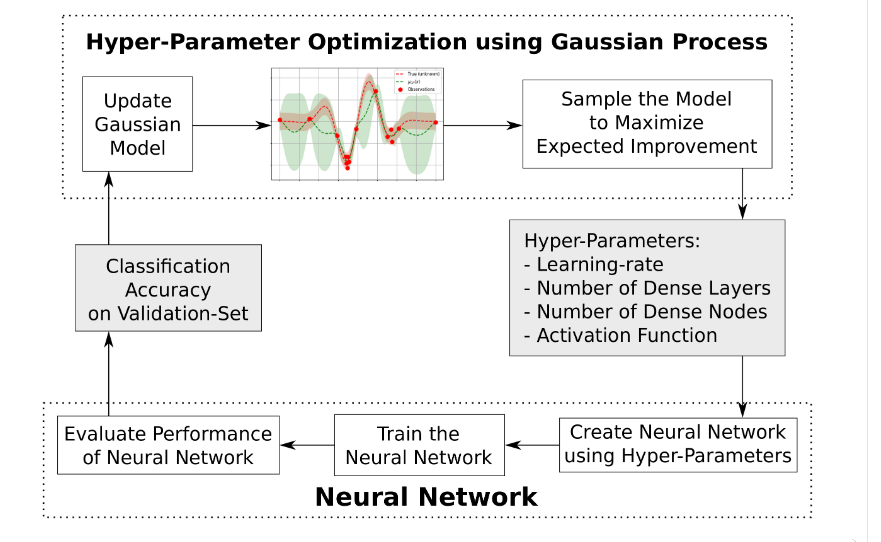
\includegraphics[width=0.75\textwidth]
            {content/graphics/applications/automl.png}
        \caption{Framework for AutoML from \emph{Achieve Bayesian optimization
            for tuning hyperparameters} by Edward Ortiz on \emph{Medium} (2020)}
    \end{figure}
\end{frame}

\begin{frame}
    \frametitle{Application: Engineering Decisions}
    \begin{figure}
        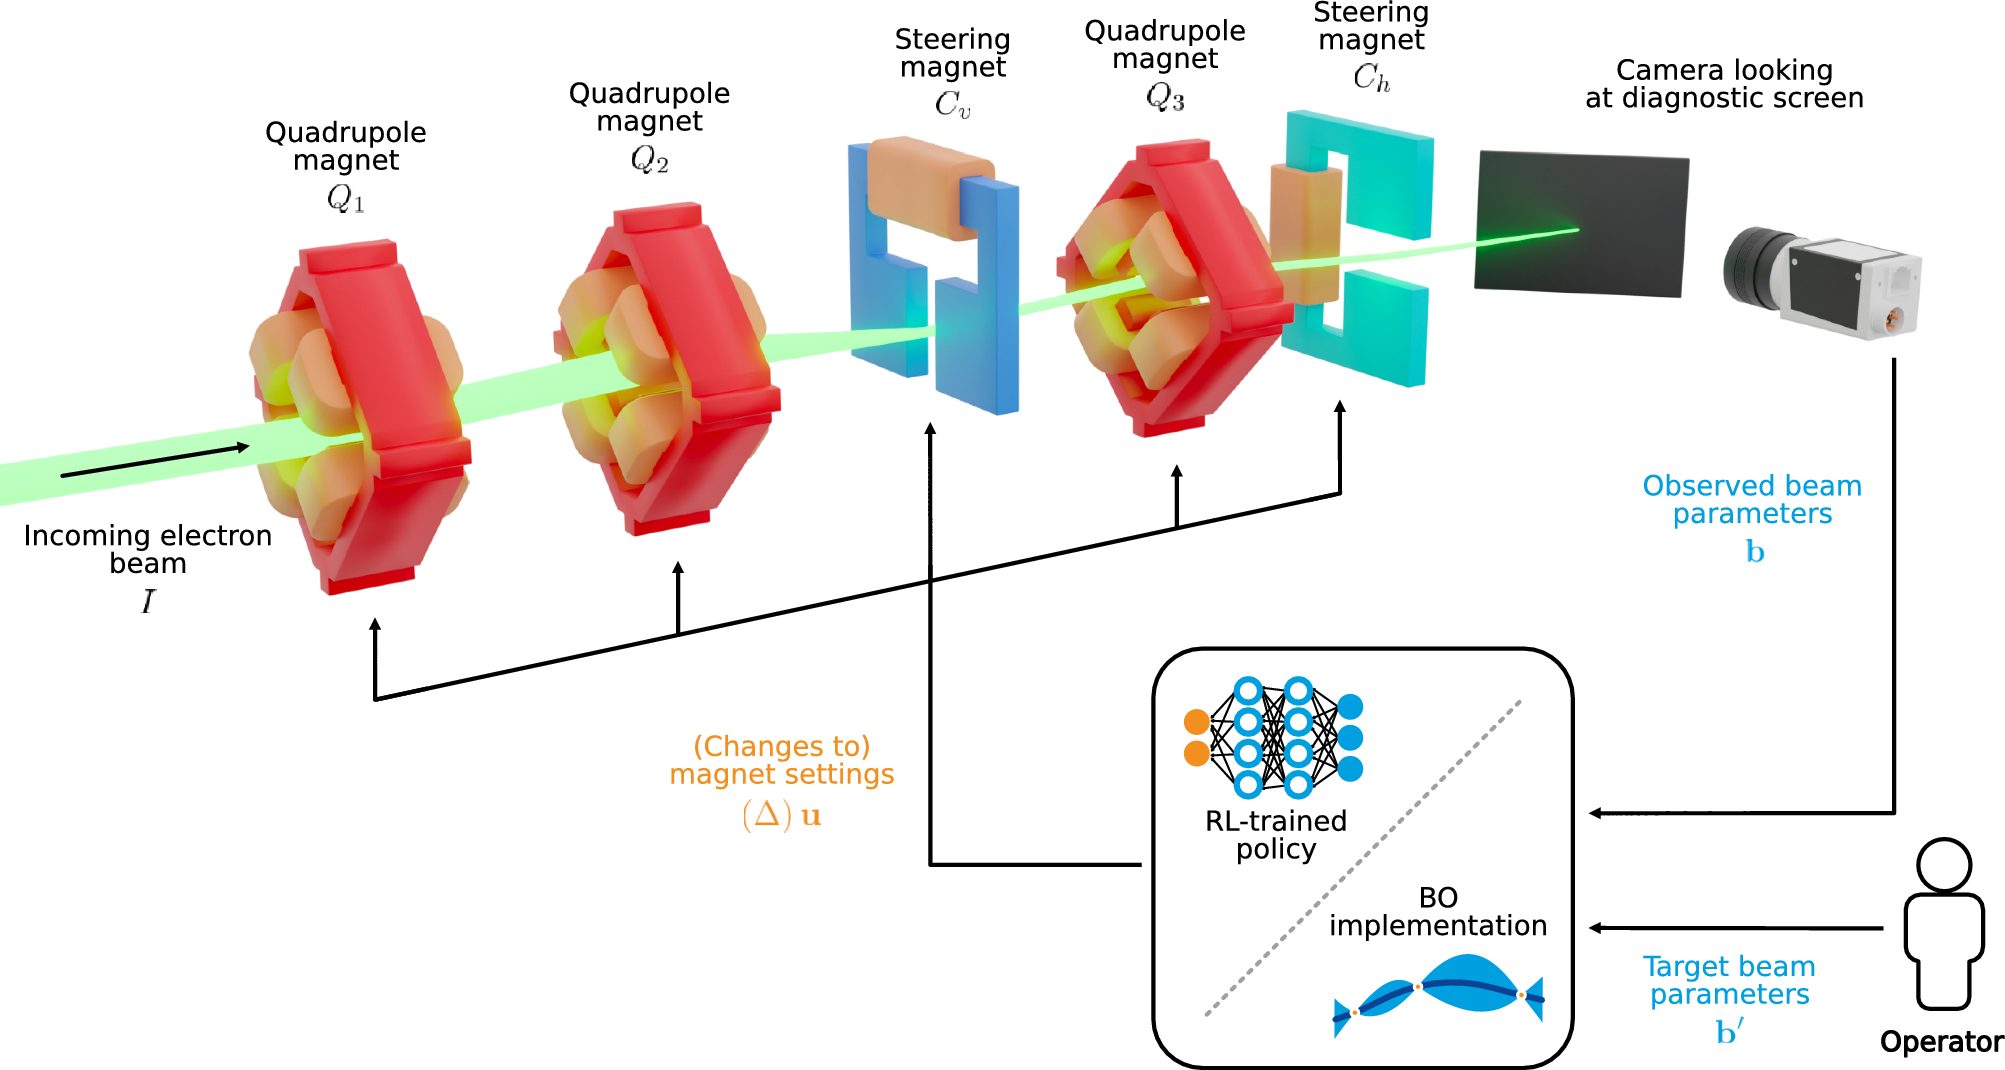
\includegraphics[width=0.85\textwidth]
            {content/graphics/applications/engineering-decisions.png}
        \caption{Framework for Particle Accelerator Tuning from
            \emph{Reinforcement learning-trained optimisers and Bayesian
            optimisation for online particle accelerator tuning} by Kaiser et
            al. (2024)}
    \end{figure}
\end{frame}